\section[User Effects]{User Effects (Søren)}
% Illustration of setup/positions on slide 1
% One slide for each:
    % All S11 on slide 2 
    % All S22 on slide 3
    % All S21 on slide 4
    % All efficiency on slide 5
    % All correlation on slide 6
    % All SAR on slide 7 (only one figure)
% For each slide, three figures/subplot (for each design)
    % Blue (freespace[0]), alpha 0.5 (min(freespace))
    % Green (data[0]), alpha 0.5 (min(data))
    % Red (play[0]), alpha 0.5 (min(play))
    % Cyan (talk[0]), alpha 0.5 (min(talk))

\def\legendfooter{\scriptsize{(1) Monopole (2) Triangle-feed (3) Dual-feed. \textcolor{bb}{Free-space}, \textcolor{gg}{Data}, \textcolor{rr}{Play}, \textcolor{cc}{Talk}. Frequency in MHz.}}
\def\emptyline{\textcolor{white}{Empty}}
\begin{frame}
    \frametitle{User Effects}
    \begin{columns}[onlytextwidth,T]
        \column{0.49\linewidth}
        Color codes: \vspace{0pt}
        \begin{tabular}{m{1in}m{3in}}
            \rule{0in}{0.3in} & \textcolor{bb}{Free space}\\
            \centering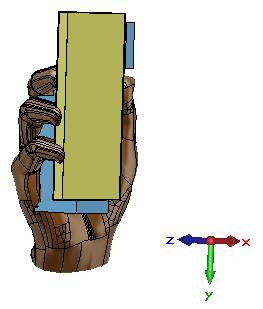
\includegraphics[height=0.6in, keepaspectratio]{img/soren/ue/usereff_onehand} & \textcolor{gg}{Data mode} \\
            \centering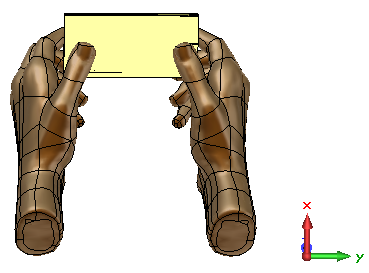
\includegraphics[height=0.6in, keepaspectratio]{img/soren/ue/usereff_twohand} & \textcolor{rr}{Play mode} \\
            \centering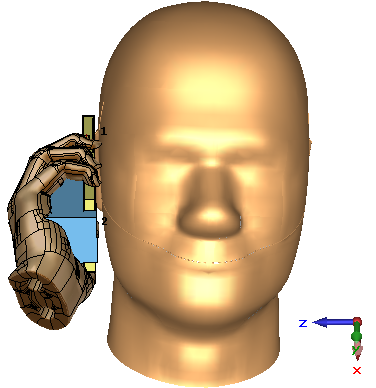
\includegraphics[height=0.6in, keepaspectratio]{img/soren/ue/usereff_headhand}& \textcolor{cc}{Talk mode}\\
            \centering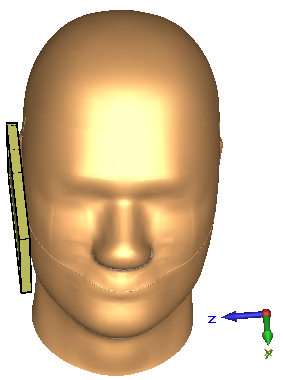
\includegraphics[height=0.6in, keepaspectratio]{img/soren/ue/usereff_sar}     & SAR
        \end{tabular}

        \column{0.49\linewidth}
        Goal:
        \begin{itemize}
            \item Find the most stable design.
            \item Preserves bandwidth in use cases.
        \end{itemize}

        Plots:
        \begin{itemize}
            \item $S_{11}$, $S_{22}$, efficiency, correlation.
            \item All SAR $<\SI{2}{W/kg}$ @ \SI{10}{g} averaging.
            \item Isolation not shown. See report.
        \end{itemize}
        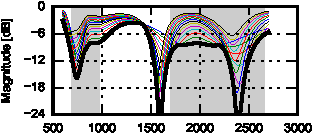
\includegraphics{img/soren/ue/design2sn/example}

        Spoiler:
        \begin{itemize}
            \item Design 2 (triangle feed) is better.
        \end{itemize}
    \end{columns}
\end{frame}

\begin{frame}
    \frametitle{User Effects -- S11, minimum over tunable range}
    % \emptyline
    Design 2 is generally is better matched.
    \begin{center}
        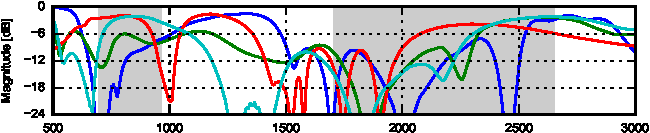
\includegraphics{img/soren/ue/design1lt/s11top.pdf}\\
        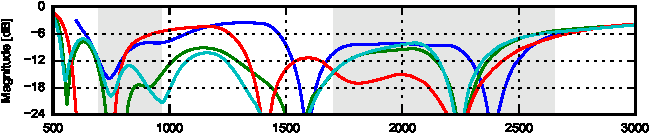
\includegraphics{img/soren/ue/design2sn/s11top.pdf}\\
        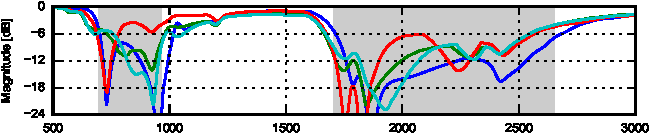
\includegraphics{img/soren/ue/design3hv/s11top.pdf}
    \end{center}
    \legendfooter
\end{frame}

\begin{frame}
    \frametitle{User Effects -- S22, minimum over tunable range}
    % \emptyline
    Detuning. Design 2 is better matched.
    \begin{center}
        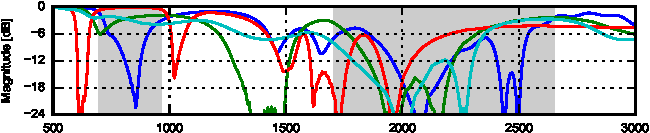
\includegraphics{img/soren/ue/design1lt/s22side.pdf}\\
        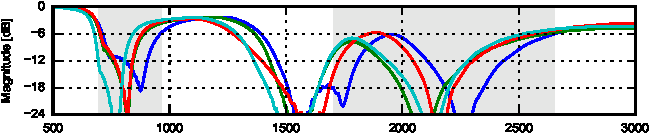
\includegraphics{img/soren/ue/design2sn/s22side.pdf}\\
        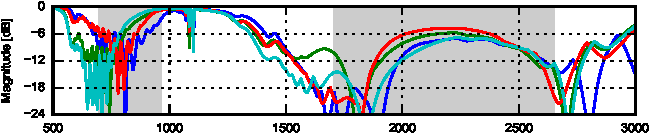
\includegraphics{img/soren/ue/design3hv/s22side.pdf}
    \end{center}
    \legendfooter
\end{frame}

\begin{frame}
    \frametitle{User Effects -- Total efficiency, minimum over tunable range (top)}
    % \emptyline
    \textit{Ideal components}. Talk mode is the worst.
    \begin{center}
        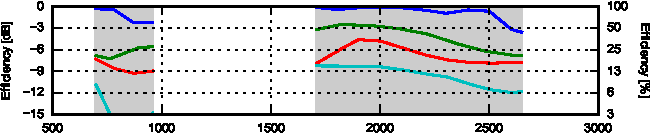
\includegraphics{img/soren/ue/design1lt/efftop.pdf}\\
        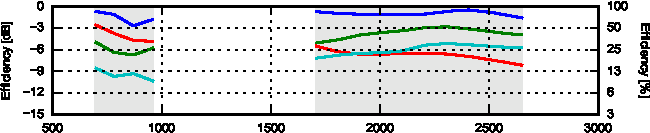
\includegraphics{img/soren/ue/design2sn/efftop.pdf}\\
        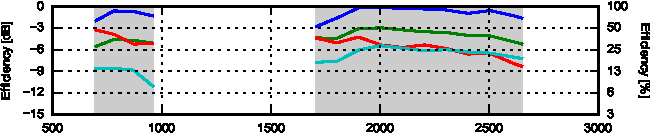
\includegraphics{img/soren/ue/design3hv/efftop.pdf}
    \end{center}
    \legendfooter
\end{frame}

\begin{frame}
    \frametitle{User Effects -- Total efficiency, minimum over tunable range (side)}
    \emptyline
    \begin{center}
        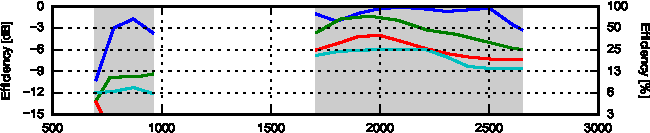
\includegraphics{img/soren/ue/design1lt/effside.pdf}\\
        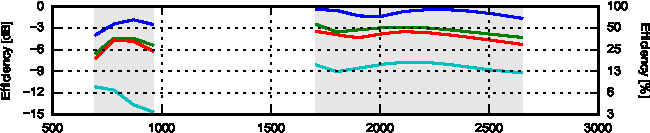
\includegraphics{img/soren/ue/design2sn/effside.pdf}\\
        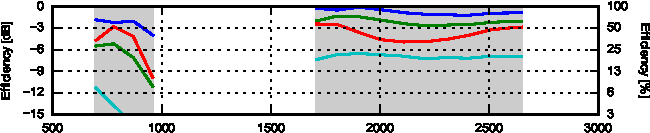
\includegraphics{img/soren/ue/design3hv/effside.pdf}
    \end{center}
    \legendfooter
\end{frame}

\begin{frame}
    \frametitle{User Effects -- Correlation, minimum over tunable range (tuning top)}
    Highest: Free-space, talk mode. Winner $=$ design 3.
    % \emptyline
    \begin{center}
        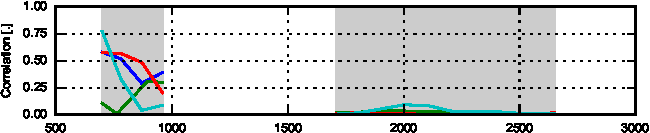
\includegraphics{img/soren/ue/design1lt/corrtop.pdf}\\
        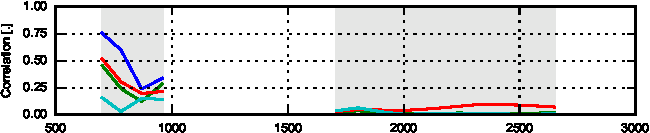
\includegraphics{img/soren/ue/design2sn/corrtop.pdf}\\
        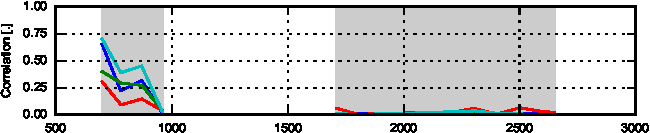
\includegraphics{img/soren/ue/design3hv/corrtop.pdf}
    \end{center}
    \legendfooter
\end{frame}

\begin{frame}
    \frametitle{User Effects -- Correlation, minimum over tunable range (tuning side)}
    Lower than tuning top.
    \emptyline
    \begin{center}
        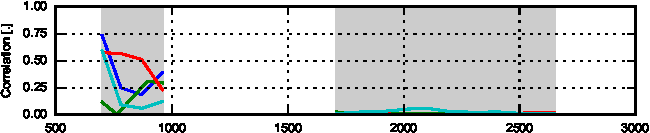
\includegraphics{img/soren/ue/design1lt/corrside.pdf}\\
        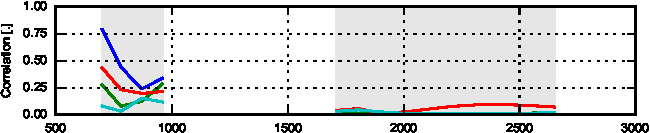
\includegraphics{img/soren/ue/design2sn/corrside.pdf}\\
        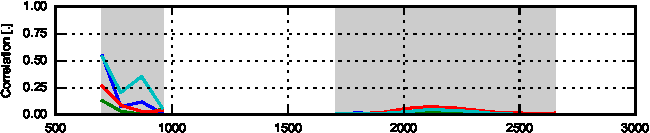
\includegraphics{img/soren/ue/design3hv/corrside.pdf}
    \end{center}
    \legendfooter
\end{frame}

\begin{frame}
    \frametitle{User Effects -- Preliminary Conclusion}
    \begin{tabular}{m{0.4in}m{4in}}
        \rule{0pt}{0.9in}
\includegraphics[height=0.75in]{img/soren/1st.pdf} & 
            Design 2 -- triangle-feed
            \begin{itemize}
                \item Better efficiency and impedance bandwidth.
                \item High free-space correlation in low band. 
            \end{itemize}
            \\
        \rule{0pt}{0.9in}
\includegraphics[height=0.75in]{img/soren/2nd.pdf} & 
            Design 3 -- dual-feed
            \begin{itemize}
                \item More fluctuating than design 2.
                \item Still good bandwidth/efficiency.
            \end{itemize}
            \\
        \rule{0pt}{0.9in}
\includegraphics[height=0.75in]{img/soren/3rd.pdf} & 
            Design 1 -- monopole
            \begin{itemize}
                \item Very sensitive to user effects.
                \item Low efficiency and impedance bandwidth.
            \end{itemize}
    \end{tabular}
\end{frame}

\section[Prototypes]{Prototypes (Søren)}
\begin{frame}
    \frametitle{Prototypes}
    \begin{columns}[onlytextwidth,T]
        \vspace{0em}
        \column{0.49\linewidth}
        \begin{tabular}{m{0.3in}m{1.4in}}
             (1) & 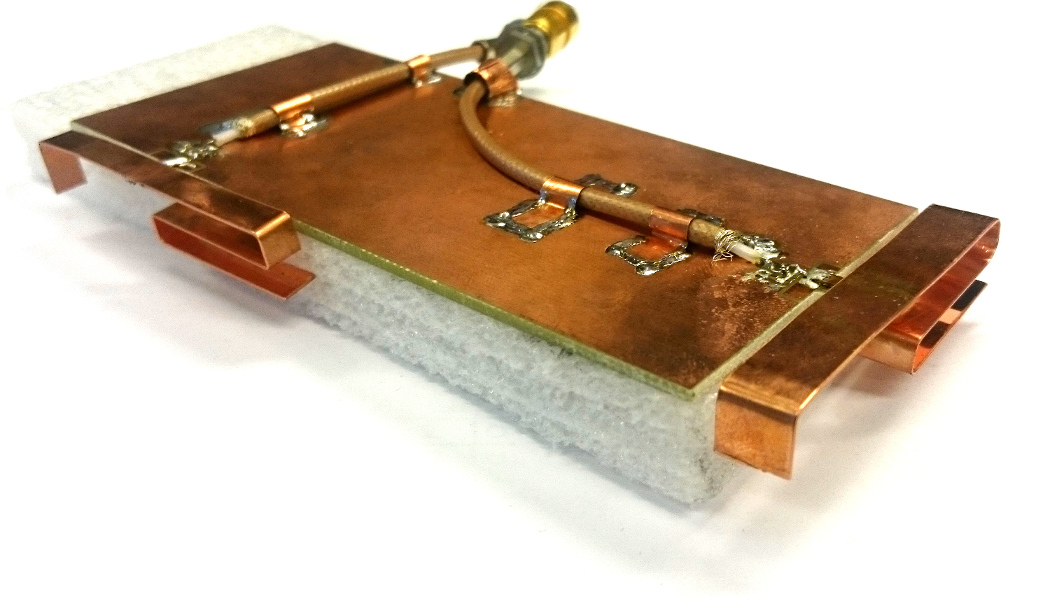
\includegraphics[width=1.4in]{img/soren/proto/design1}\\
             (2) & 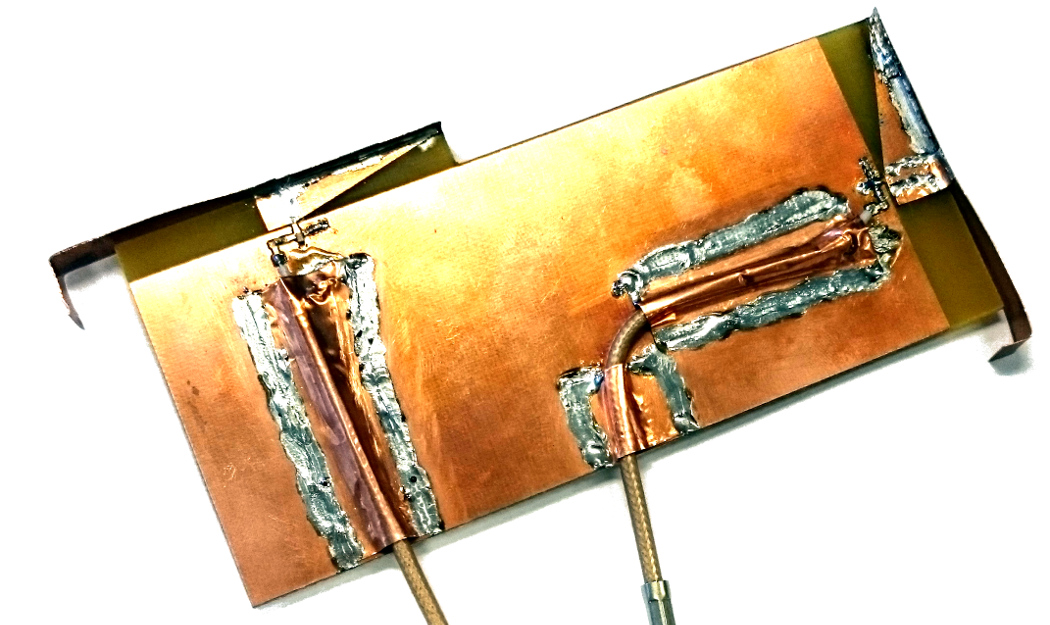
\includegraphics[width=1.4in]{img/soren/proto/design2}\\
             (3) & 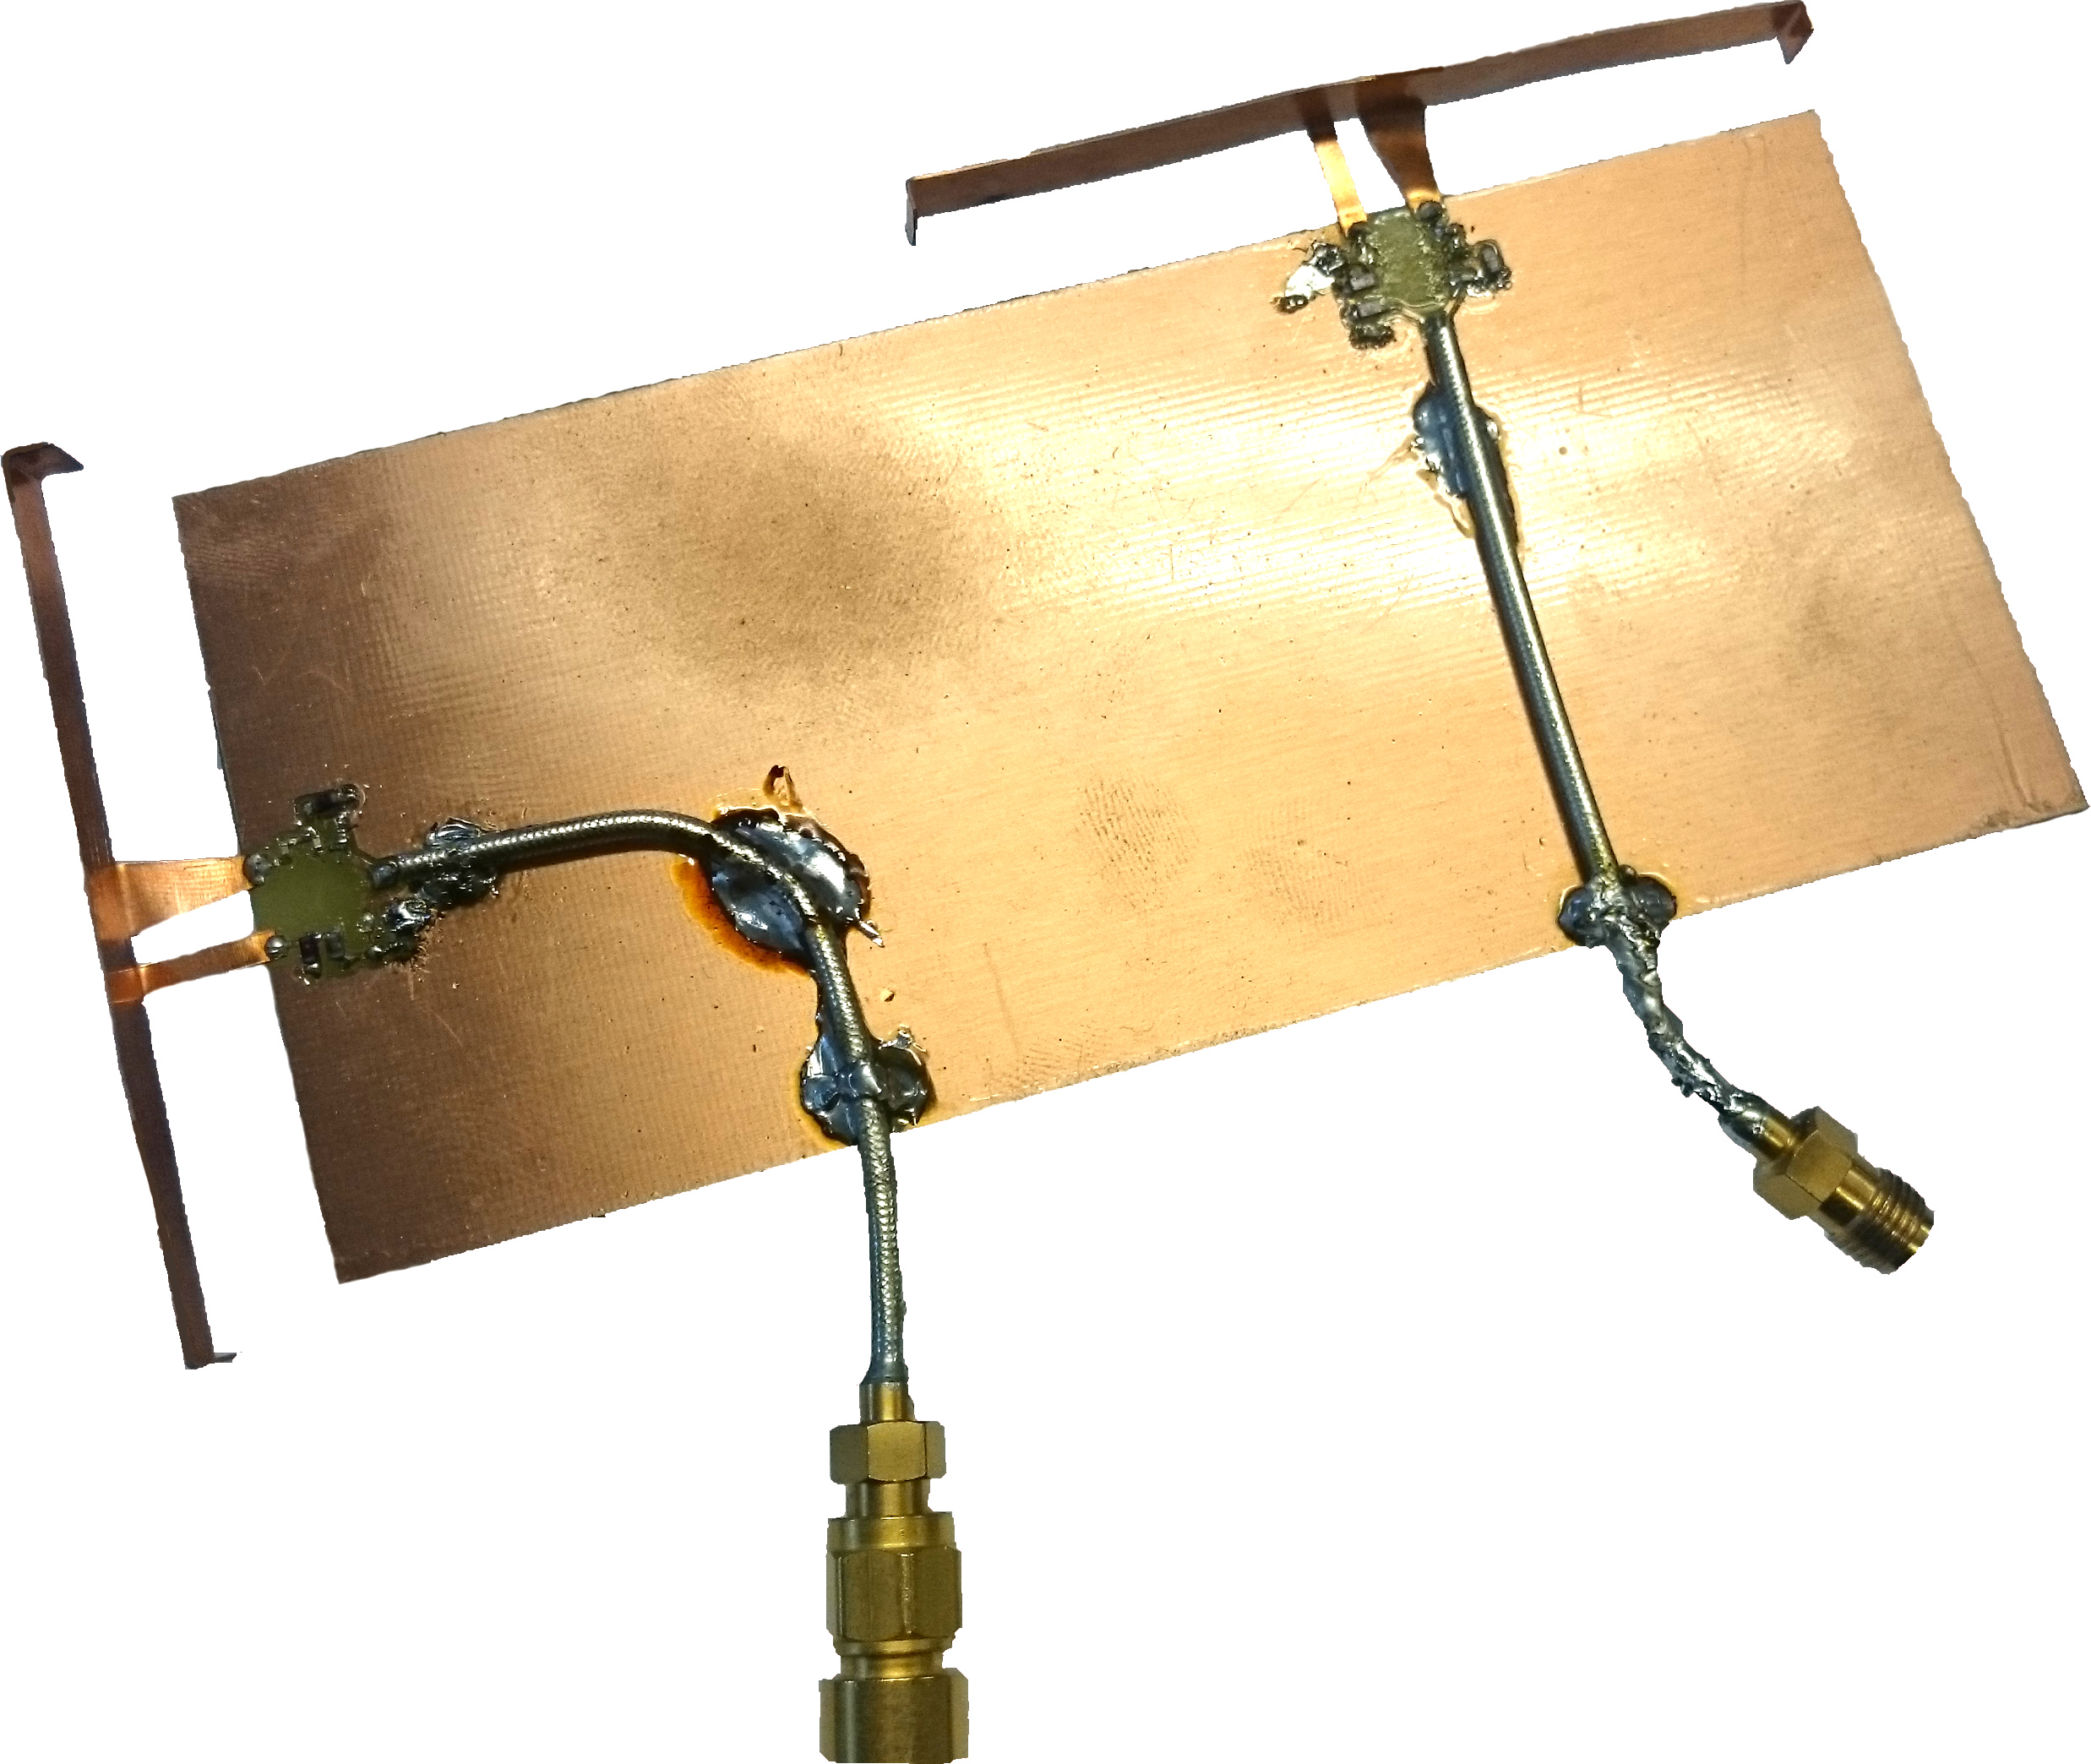
\includegraphics[width=1.4in]{img/soren/proto/design3}
        \end{tabular}

        \column{0.49\linewidth}
        Goal:
        \begin{itemize}
            \item Find most realizable design.
            \item Verify simulation results -- useful design in real life?
        \end{itemize}

        Plots:
        \begin{itemize}
            \item $S_{11}$, $S_{22}$, efficiency.
            \item Isolation not shown. See report.
        \end{itemize}

        Spoiler:
        \begin{itemize}
            \item Design 2 (triangle-feed) is better.
        \end{itemize}
    \end{columns}
\end{frame}

\def\legendfooter{\scriptsize{Upper: Top antenna. Lower: Side antenna. Frequency in MHz.}}
\begin{frame}
    \frametitle{Prototype 1 -- Monopole}
    High band moves a lot during tuning.
    % \emptyline
    \begin{center}
        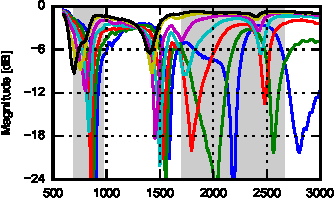
\includegraphics{img/soren/proto/design1lt/s11.pdf}
        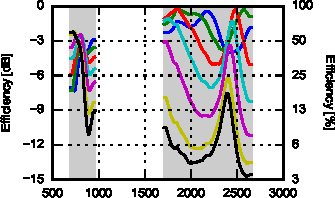
\includegraphics{img/soren/proto/design1lt/efftop.pdf}\\
        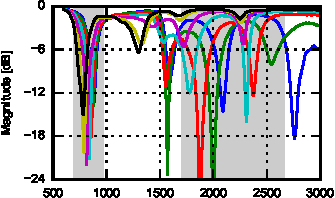
\includegraphics{img/soren/proto/design1lt/s22.pdf}
        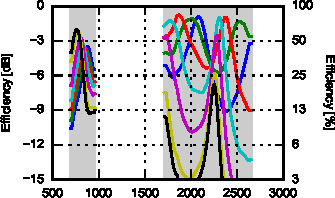
\includegraphics{img/soren/proto/design1lt/effside.pdf}
    \end{center}
    \legendfooter
\end{frame}

\begin{frame}
    \frametitle{Prototype 2 -- Triangle-feed}
    \textcolor{gg}{High bandwidth!} High band stable over multiple capacitances.
    % \emptyline
    \begin{center}
        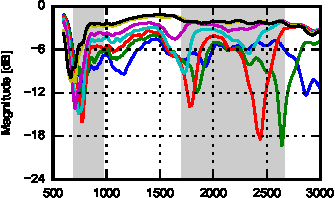
\includegraphics{img/soren/proto/design2sn/s11.pdf}
        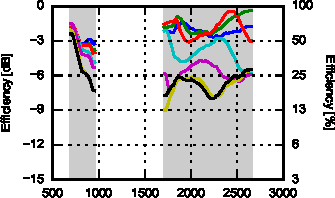
\includegraphics{img/soren/proto/design2sn/efftop.pdf}\\
        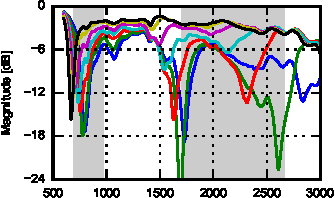
\includegraphics{img/soren/proto/design2sn/s22.pdf}
        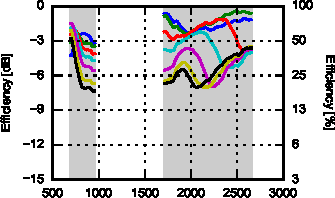
\includegraphics{img/soren/proto/design2sn/effside.pdf}
    \end{center}
    \legendfooter
\end{frame}

\begin{frame}
    \frametitle{Prototype 3 -- Dual-feed}
    OK efficiency. Side antenna -- good but not tunable.
    % \emptyline
    \begin{center}
        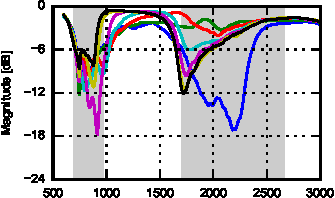
\includegraphics{img/soren/proto/design3hv/s11.pdf}
        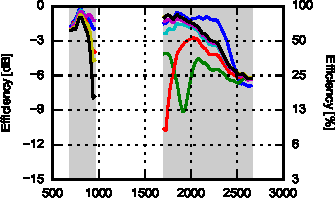
\includegraphics{img/soren/proto/design3hv/efftop.pdf}\\
        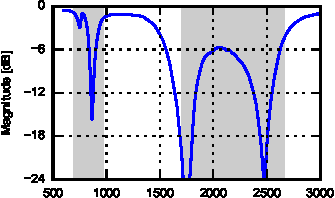
\includegraphics{img/soren/proto/design3hv/s22.pdf}
        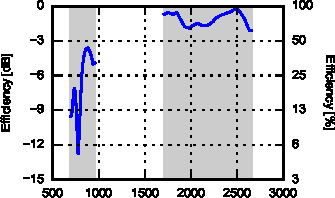
\includegraphics{img/soren/proto/design3hv/effside.pdf}
    \end{center}
    \legendfooter
\end{frame}

\begin{frame}
    \frametitle{Prototypes -- Preliminary Conclusion}
    \begin{tabular}{m{0.4in}m{4in}}
        \rule{0pt}{0.9in}
\includegraphics[height=0.75in]{img/soren/1st.pdf} & 
            Design 2 -- triangle-feed.
            \begin{itemize}
                \item Covers all bands at $C_{\text{low}}$.
                \item Preserves higher efficiency when tuned.
                \item \textit{Moved to tuner PCB}.
            \end{itemize}
            \\
        \rule{0pt}{0.9in}
\includegraphics[height=0.75in]{img/soren/2nd.pdf} & 
            Design 3 -- dual-feed
            \begin{itemize}
                \item Top antenna good in most bands.
                \item Side antenna not tunable but good.
                \item Matching network $\neq$ tuner PCB.
            \end{itemize}
            \\
        \rule{0pt}{0.9in}
\includegraphics[height=0.75in]{img/soren/3rd.pdf} & 
            Design 1 -- monopole
            \begin{itemize}
                \item Covers low bands OK.
                \item Low efficiency when tuned.
            \end{itemize}
    \end{tabular}
\end{frame}
